% Chapter Template

\chapter{Optical Testbed} % Main chapter title
\noindent\textbf{\large Contents:}

\noindent\hrulefill
\noindent\startcontents[chapters]
\noindent\printcontents[chapters]{}{1}{}
\noindent\hrulefill
\label{Chapter3} % Change X to a consecutive number; for referencing this chapter elsewhere, use \ref{ChapterX}
% \tableofcontents

% \vspace{5mm}


With the simulation work done showing that we can indeed do focal plane wavefront sensing on the GMT pupil with a vAPP, we now must show that we can do FPWFS on the optical bench.

\section{Optical Layout}
\label{sec:optical_layout}

The goals of the optical testbed were to simulate piston, tip, and tilt onto each segment of the GMT pupil using a deformable mirror (DM).  So the constraints of our optical system were to match the size of the DM and then zoom onto the GMT vAPP.  First step was to couple a 532nm laser to a single mode optical fiber.  As the laser light leaves the fiber, it will diverge.  The light is collimated using an achromat onto an 11mm circular aperture.  The aperture size was dependant on the aperture size of the DM and made slightly undersized in order to avoid the DM edge actuators which tend to not perform reliably.  With the entrance pupil (EP) set, the achromats need to have a 1:1 relay of the pupil plane onto the DM.  Therefore they were all set to the same focal length.


\begin{figure}[H]
    \centering
    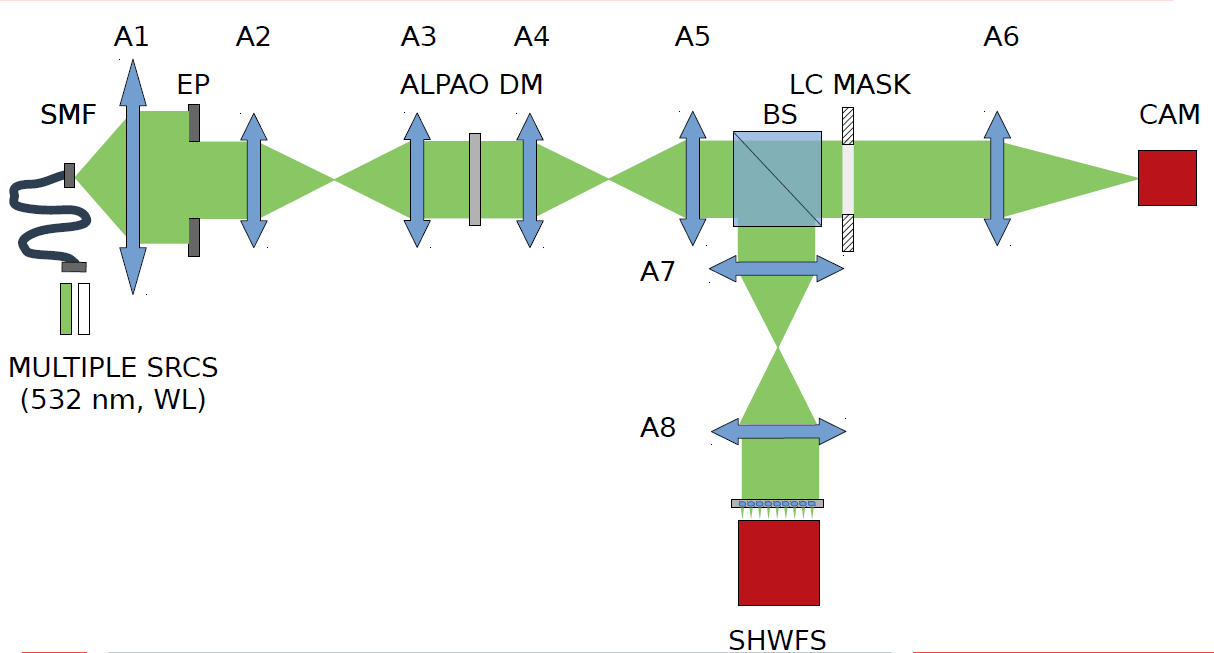
\includegraphics[width = 12cm]{Figures/optical_bed.png}
    \caption{Paraxial view of the GMT testbed}
    \label{fig:optical_layout}
\end{figure}

After the DM, there needed to be a $\approx$ 1:2 relay in order to zoom the pupil from the 11mm DM aperture to the $\approx 6$mm vAPP aperture on the LC Mask.  Then from the vAPP, the last achromat needed to have a long enough focal length to Nyquist sample the Airy core of the PSF.  Before the LC MASK, a beam splitter was put in to direct light to a Shack-Hartmann wavefront sensor.  This was so that verification of the aberrated wavefront was possible.  The decision to use achromats rather than monochromatic lenses was made so that other projects could use other wavelengths for their purposes.  However, our vAPP was tuned to 532nm.  Figure \ref{fig:optical_layout} shows a paraxial design of the described layout.  However, due to technical difficulties and with the addition of the current pandemic, the DM was replaced by a simple fold mirror.


\section{Optical Alignment}

Because the purpose of the optical bench was to do wavefront measurements, optical aberrations were to be kept to a minimum.  This meant going through a rigorous alignment procedure.  Initially we set up the optical bench to a rough approximation of the focal distances to get the total size of the layout.  Then each optic position was marked and removed.  A few Iris's was mounted to a post and measured the height of the outgoing light from the fiber optic.  This was so that we could keep a continuous height through out the entire system.  Next first achromat (A1) was put back in the system.  In order to properly collimiate the light path, we used a shear plate interferometer.  How a shear plate interferometer works, is that as light passes through a 45 degree angle window, part of the light is reflected on each surface.  A diagram of this can be seen in Figure \ref{fig:shearplate}.


\begin{figure}[H]
\centering
\begin{subfigure}{.5\textwidth}
  \centering
  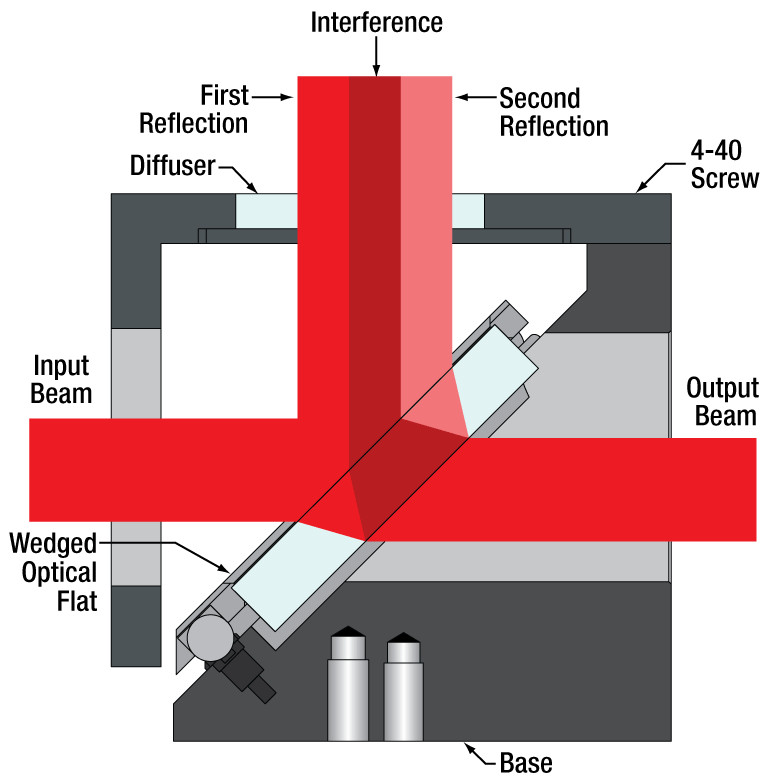
\includegraphics[width=6.5cm]{Figures/ShearPlateDrawing.jpg}
  \caption{Diagram of how a shear plate interferometer works \cite{ShearingInterferometers}.}
  \label{fig:shearplate}
\end{subfigure}%
\begin{subfigure}{.5\textwidth}
  \centering
  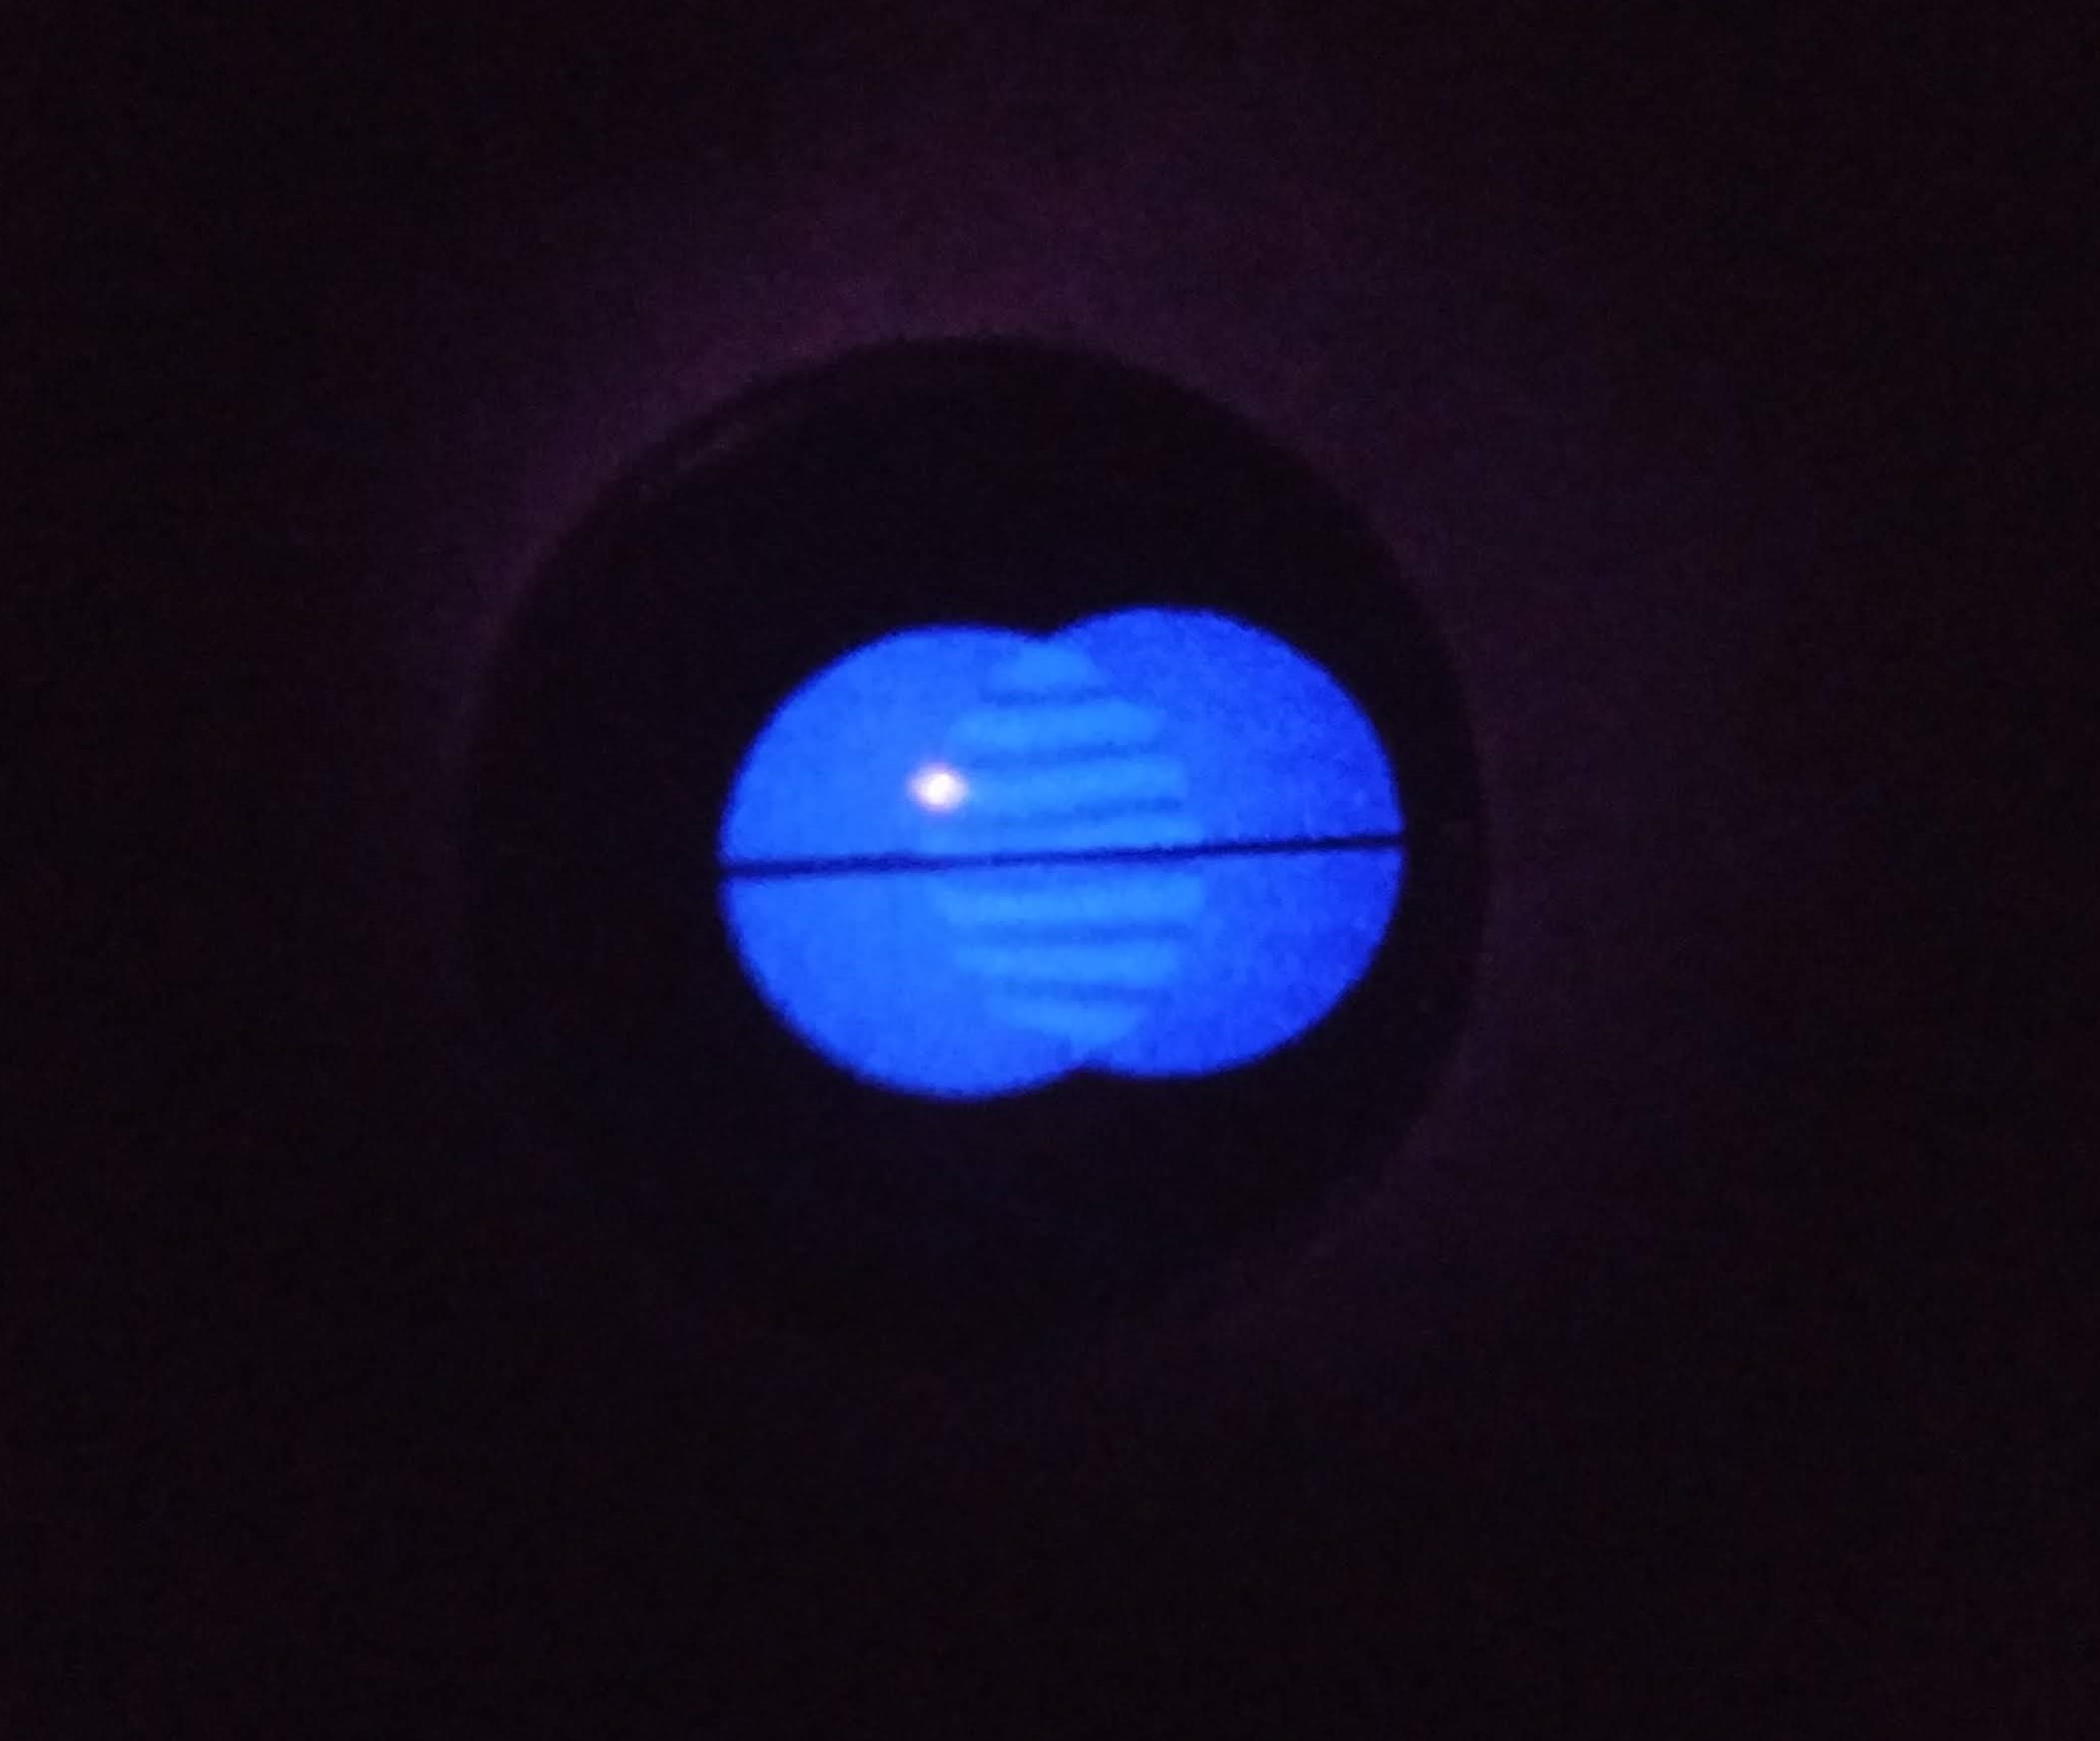
\includegraphics[width=7cm]{Figures/fringes.jpg}
  \caption{Fringe pattern of the shear plate interferometer.}
  \label{fig:fringes}
\end{subfigure}
\caption{Shear plate interferometer examples.}
\label{fig:shear_images}
\end{figure}

The first reflection interferes with the second reflection to cause an interference patter like the one in Figure \ref{fig:fringes}.  When the fringe pattern is at a tilt, then the beam is either converging or diverging (Figure \ref{fig:shear_read}).  It is also possible to view other aberrations with a shear plate interferometer.  As seen in Figure \ref{fig:fringes}, the lines have a slight curve on the left hand side of the window.  This could possibly mean that there is some spherical aberrations in our system.  All of the achromats are spherical optics so this is something we can only try to minimize and then move on. 


\begin{figure}[H]
    \centering
    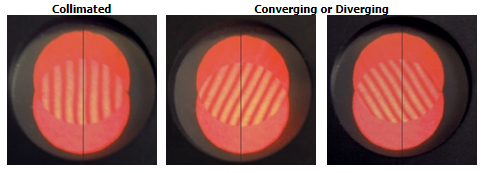
\includegraphics[width = 10cm]{Figures/shear_coll.png}
    \caption{Example of how to read a shear plate interferometer \cite{ShearingInterferometers}}
    \label{fig:shear_read}
\end{figure}

With the beam collimated, the reference iris was placed in the system to ensure that the height of the beam had not changed.  Next was to do a near/far test with the iris.  The near/far test can be used to approximate collimation, however we used this test to make sure that the light path was always pointing straight and not diverting light off at an angle.  When we were satisfied that the light was properly collimated and pointing correctly, the entrance pupil was mounted.  It was essential that the entrance pupil be at the center of the light column as well.  Laser light leaving the fiber is not equally illuminated across the pupil, so if the entrance pupil was not concentric with the light column, then that could lead to additional aberrations.

Next was to refocus the light.  In order to test the focal plane a test camera was placed at the focus.  In most cases, we could simply look at the airy rings and core to determine what aberrations we are seeing.  However, the first focal plane was too fast and we were unable to proper sample the PSF.  What we were able to do was put the camera before the focal plane and move it through and past the focal plane.  The would show if there were any signs of coma or astigmatism.  This same process for collimation and focus alignment was repeated for the rest of the system.  

For the flat mirror we put in place of the DM, we needed to divert the light as little as possible to limit the tilt aberration in the system.  After we placed this pseudo-DM, we double checked the aiming and collimation using the reference iris's and shear plate interferometer.  Then a second mirror was placed to continue the light path down the reference holes in the breadboard.  


\begin{figure}[H]
\centering
\begin{subfigure}{.5\textwidth}
  \centering
  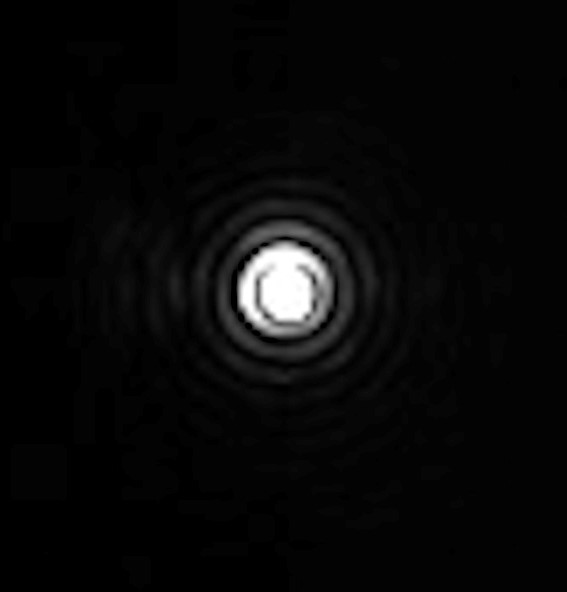
\includegraphics[width=6.5cm]{Figures/new_int_focal_plane.jpg}
  \caption{The intermittent focal plane after A4.}
  \label{fig:int_focal_plane}
\end{subfigure}%
\begin{subfigure}{.5\textwidth}
  \centering
  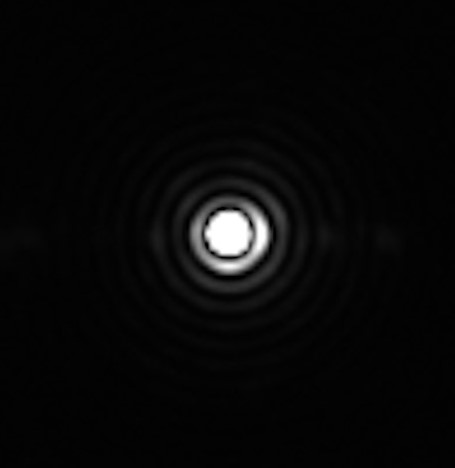
\includegraphics[width=7cm]{Figures/final_focal.jpg}
  \caption{Final focal plane.}
  \label{fig:final_focal}
\end{subfigure}
\caption{Focal plane images}
\label{fig:focal_images}
\end{figure}


\section{Images \& Wavefront Decomposition}